\subsection{Discussion}

\begin{figure}
\center
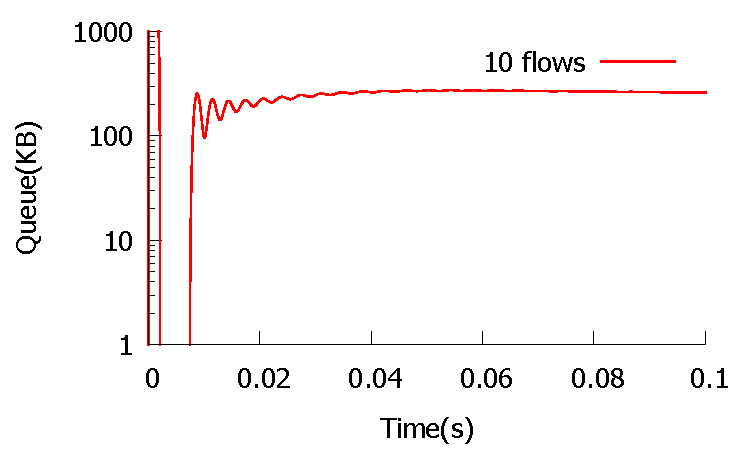
\includegraphics[width=0.33\textwidth]{figures/stable_q_85_pi.pdf}
\caption{PI marking scheme can stabilize DCQCN}
\label{fig:dcqcn_pi}
\end{figure}

\para{Using PI controller for enhanced stability:}
A more principled appraoch to stabilizing DCQCN for all operating regimes is to
use a PI~\cite{Hollot:PIController}-based packet marking scheme, instead of the
RED-like marking scheme of Equation (\ref{eq:mark}). We are currently
investigating this option in more detail; a sample result is shown in
Figure~\ref{fig:dcqcn_pi}. One important advantage of the using the PI
controller is that the staedy-state queue length is indepedent of the number of
flows.


%DCQCN is stable at 100Gbps even when the control loop delay is $100\mu s$. TODO:
%similar for the PI controller. We conclude that DCQCN easily adapts to higher
%bandwidth fabrics with minor tunings. 

